\section{Durchführung}
\label{sec:Durchführung}

\subsection{Versuchsaufbau}
\label{sec:Versuchsaufbau}
%\begin{figure}
%	\centering
%	\caption{Schematische Darstellung des Versuchsaufbaus \cite{anleitung}.}
%	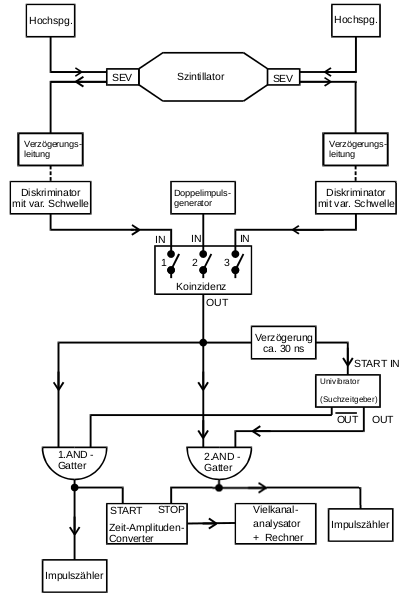
\includegraphics{Bilder/aufbau.png}
%	\label{fig:aufbau}
%\end{figure}
%
%\begin{figure}
%	\centering
%	\caption{Schematische Darstellung der Quelle zur Erzeugung radioaktiven Isotopen \cite{anleitung}.}
%	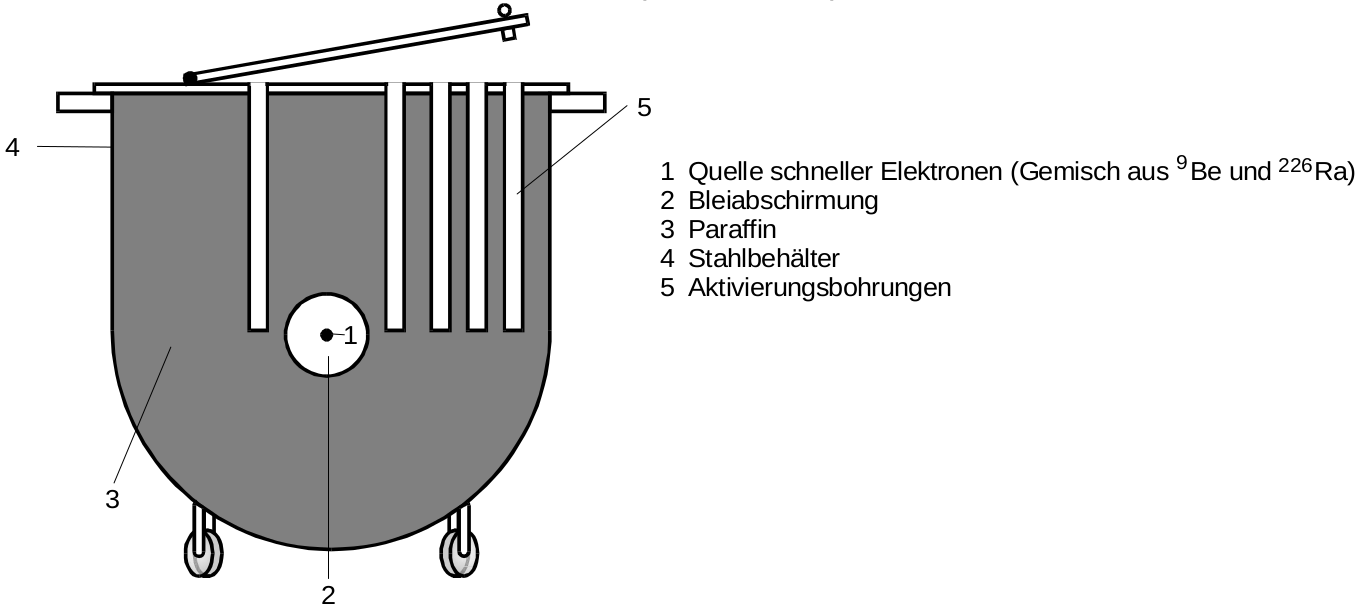
\includegraphics{content/toepfchen.png}
%	\label{fig:kochen}
%\end{figure}
%
Der Versuchsaufbau -- wie in Abbildung \ref{fig:aufbau} dargestellt -- besteht im Wesentlichen 
aus einem zerfallenden radioaktiven Isotop und einem Geiger-Müller-Zählrohr, welches die 
zerfallenden Kerne misst.
Das Geiger-Müller-Zählrohr ist entspricht einer mit Gas gefüllten Röhre. Trifft ein $\beta$-
oder $\gamma$- Teilchen auf ein Gasteilchen wird dieses ionisiert und kann aufgrund einer
anliegenden Spannung an der Röhre gemessen werden.
Dabei werden die gemessenen Zerfälle pro Messzeitintervall, welches am Zeitgeber einstellbar 
ist, an den Zählern 1 und 2 angezeigt. Nach jedem Messvorgang wird der Zähler umgeschaltet und 
der vorherige Wert auf dem aktuellen Zähler wird überschrieben. Der Versuchsaufbau ist mit
einer Blei-Abschirmung ausgestattet um die radioaktive Strahlung abzuschirmen.

Zur Erzeugung der radioaktiven Isotope wird das Objekt in Abbildung \ref{fig:kochen} verwendet.
Hierbei werden stabile Kerne mit niederenergetischen Neutronen beschossen. 
Da die Neutronen ihre Energie durch elastische Stöße an die Kerne übergeben und die maximale
Energie bei gleichen Massen der Stoßpartner erreicht wird, werden die Neutronen in einem 
Paraffinmantel gebremst, bis sie die optimale Energie besitzen.


\subsection{Versuchsbeschreibung}
\label{sec:Versuchsbeschreibung}


\subsubsection{Messung zur Verifizierung der Gleichungen}

Für die Verifizierung der Gleichungen \eqref{eqn:abbi} und \eqref{eqn:linsi} wird der
Aufbau wie in Abschnitt \ref{sec:gundb} mit einer Sammellinse der Brennweite
\SI{100}{\milli\meter} verwendet.\\
Zu Beginn wird die Gegenstandgröße $G$ - die Größe des "Perl L"s - mit dem Lineal gemessen.
Daraufhin werden für zehn Gegenstandsweiten $g$ die Bildweiten $b$ bestimmt, bei denen auf dem
Schirm ein scharfes reelles Bild zu erkennen ist. Hierfür soll der Schirm verschoben werden.
Des Weiteren werden für die ersten fünf Messungen außerdem die Bildgrößen auf dem Schirm mit
einem Lineal bestimmt. Es werden also zehn Wertepaare $(g_{\mathrm{i}},b_{\mathrm{i}})$ und
fünf Bildgrößen notiert.

\subsubsection{Messung für die unbekannte Sammellinse}

Die Messung der Brennweite der mit Wasser gefüllten Linse erfolgt analog zur vorherigen
Messung. Es werden allerdings nur zehn Wertepaare $(g_{\mathrm{i}},b_{\mathrm{i}})$
benötigt.\\
Hierbei ist zu beachten, dass ein konstanter Druck auf die Spritze ausgeübt wird,
damit das Wasservolumen in der Linse konstant bleibt.

\subsubsection{Messung für die Methode nach Bessel}
\begin{figure}
  \centering
  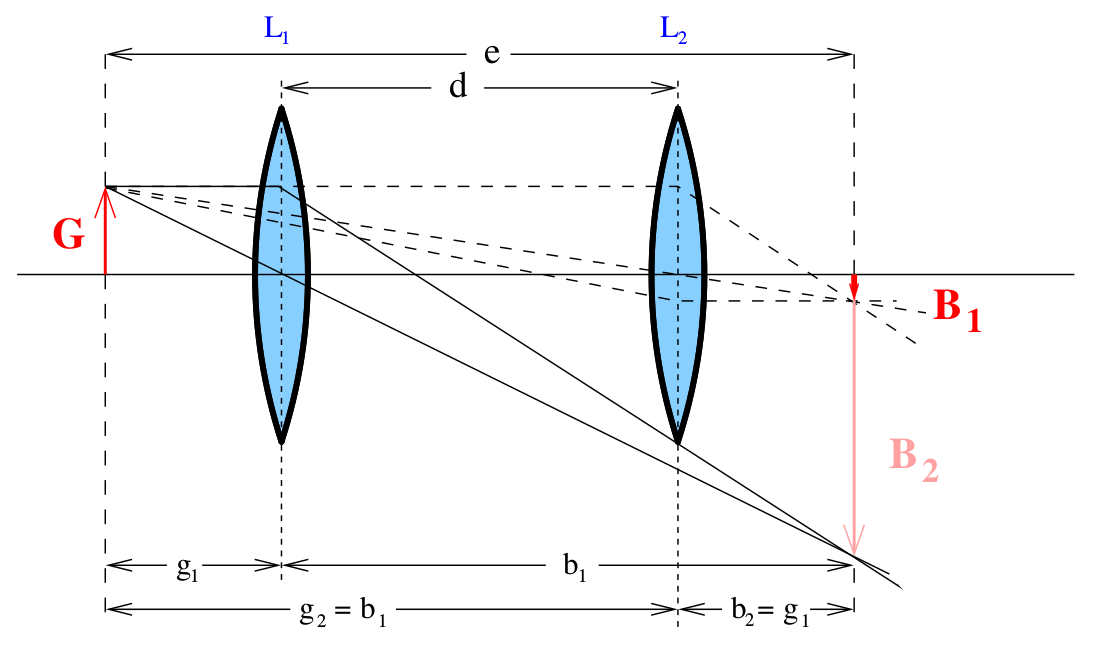
\includegraphics[width=0.6\textwidth]{Bilder/Bessel.png}
  \caption{Schematische Darstellung der beiden Linsenpositionen an denen ein scharfes Bild auf dem Schirm entsteht zur Bestimmung der Brennweite nach der bessel-Methode.}
  \label{fig:besselmess}
\end{figure}
Bei der Messung für die Methode nach Bessel wird wieder die Linse mit der Brennweite
$f=\SI{100}{\milli\meter}$ angebracht.
Dann wird der Abstand zwischen Gegenstand und Schirm festgehalten und die Linse solange variiert
bis beide Punkte bestimmt sind (vgl. Abbildung \ref{fig:besselmess}) , an denen ein scharfes Bild am Schirm zu sehen ist.
Für diese beiden Punkte werden jeweils die Gegenstandsweite $g_{1,2}$ und die Bildweite
$b_{1,2}$ notiert. Diese Messung soll für zehn verschiedene Abstände von Gegenstand und Schirm
durchgeführt werden.\\
Da außerdem die chromatische Abberation untersucht werden soll, werden bei den ersten fünf
Messungen jeweils ein Rot- und ein Blaufilter angebracht und die Messung wiederholt.

\subsubsection{Messung für die Methode nach Abbe}

Für die Messung nach der Methode von Abbe wird vor der Sammellinse die Zerstreuungslinse mit
Brennweite $f_{\mathrm{Z}}=-\SI{100}{\milli\meter}$ - wie in Abschnitt \ref{sec:abbe}
beschrieben - angebracht. Der Punkt A wird als Berührungspunkt der beiden Reiter, auf denen
sich die Linsen befinden, festgelegt und die Hilfsgegenstandsweite $g'$  und Hilfsbildweite $b'$ wieder zehnmal
gemessen bis ein scharfes Bild auf dem Schirm zu erkennen ist.
